\section*{Proposta de Trabalho - Lista 01}
\begin{itemize}
\item[1)]Implementar em qualquer linguagem de programação o Exemplo 4.3 do Livro Introdução à Transferência de Calor e Massa, Incropera e DeWitt (em anexo). Resolver o exemplo exatamente como apresentado no livro, utilizando o Método das Diferenças Finitas e os mesmos doze (12) pontos nodais (malha de 0,25 m), conforme apresentado no livro:
    \begin{itemize}
        \item[a)]Verificar a sua solução com a do livro;
        
        \textbf{OBS: RESOLVER ITERATIVAMENTE}

        \item[b)]Implemente uma maneira para contabilizar o tempo necessário para o seu programa convergir;
        \item[c)]Fazer um estudo de refino de malha, utilizando um critério de convergência de $0,01\,^\circ\mathrm{C}$ (utilizando a equação apresentada na p. 141, Eq. 4.52). \uline{Selecione uma malha que você achar conveniente e justifique sua escolha;}
        \item[d)]Utilizando a malha selecionada, faça uma análise em quanto ao critério de convergência utilizando a equação apresentada na p. 141, Eq. 4.52. \uline{Selecione o critério de convergência que você achar conveniente e justifique sua escolha;}
        \item[e)]Apresente o campo de temperaturas encontrado em um gráfico 3D;
        \item[f)]Apresente o gráfico dos vetores fluxo de calor (gráfico 3D);
    \end{itemize}
\end{itemize}
\section*{Resolução}

\begin{itemize}
    \item[1) a)]Através do método de Gauss-Seidel, apresentado na página 141, pôde-se obter os mesmos valores de temperaturas apresentados no exemplo resolvido do livro.
    
    O código se encontra no ANEXO I.

    \item[b)]Utilizou-se o a função \texttt{perf\_counter()} do pacote \texttt{time} do Python para contabilização do tempo de execução do código. Iniciou-se a contagem do tempo logo antes das etapas de realização do Método de Gauss-Seidel e finalizou-se a contagem após o término de aplicação das operações. A diferença entre os tempos foi calculada, obtendo-se o tempo total necessário para execução do método.
    
    \item[c)]\subsection*{Refino de malha com $\varepsilon = 0,01\,^\circ\mathrm{C}$}
    Com base na equação $|T_{i}^{k} - T_{i}^{k-1}| \le \varepsilon$, tentou-se realizar um estudo de refino de malha utilizando-se o critério de convergência $\varepsilon \le 0,01^\circ\mathrm{C}$.

    O critério utilizado para a análise foi a avaliação do módulo da diferença dos valores de $T_7$ e $T_8$ obtidos com a malha mais refinada e os valores das mesmas temperaturas obtidas com a malha imediatamente anterior (menos refinada).
    \clearpage
        \small
        Exemplo:
        \begin{itemize}
            \item[-]Malha inicial: $\Delta x = \Delta y = 0,25\,\mathrm{m}$, $T_7 = 357,00\,^\circ\mathrm{C}$, $T_8 = 339,05\,^\circ\mathrm{C}$
            \item[-]Malha sequencial: $\Delta x = \Delta y = 0,05\,\mathrm{m}$, $T_7 = 348,58\,^\circ\mathrm{C}$, $T_8 = 337,41\,^\circ\mathrm{C}$
            
            \vspace{0.2cm}
            
            $\Delta T_7 = |357,00 - 348,58| = 8,42\,\mathrm{^\circ\mathrm{C}}$ 

            $\Delta T_8 = |339,05 - 337,41| = 1,64\,\mathrm{^\circ\mathrm{C}}$        
        \end{itemize}
    Tais critérios foram utilizados, pois esses são os pontos críticos do problema. Os pontos estão situados em uma das regiões de contorno do objeto de estudo e são os únicos submetidos à condução e à convecção simultaneamente.

    Foram avaliadas 6 malhas com diferentes níveis de refinamento. A malha inicial possuía elementos quadrados de lado $0,25\,\mathrm{m}$. Para cada nível de refinamento $n$ (múltiplos de 5), o comprimento dos elementos foi determinado pela relação:
    \begin{center}
        $\Delta x = \Delta y =  \dfrac{0,25}{n}\,\mathrm{m}$,\quad $n = \{1, 5, 10, 15, 20, 25\}$
    \end{center}

    E o número de elementos da malha foi determinado pela relação:
    \begin{center}
        $n_{elementos} = \left[ \dfrac{1}{\Delta x} \right]^{2}$
    \end{center}

    Além disso, adotou-se o critério de $\Delta T \le 0,2\;^\circ\mathrm{C}$ em relação a ambas as temperaturas $T_7$ e $T_8$ como tolerância quanto ao estabelecimento da hipótese de independência de malha.

    Dessa forma, ao analisar os resultados dos valores de $\Delta T_7$ e $\Delta T_8$ em relação aos números de elementos da malha, notou-se, inicialmente, que as diferenças de temperatura diminuiram bruscamente, alcançando um mínimo para $n_{elementos} = 1600$ ($\Delta x = 0,025\,\mathrm{m}$), inclusive, apresentando um valor de $\Delta T$ inferior ao critério estabelecido de independência de malha para a temperatura $T_7$, porém, não para a temperatura $T_8$, invalidando a hipotese. Além do mais, os valores de $\Delta T$ voltaram a crescer a medida que o $n_{elementos}$ também aumentava.
    
    Percebeu-se também, que o esforço computacional se elevava consideravelmente a cada iteração.

    Os valores das temperaturas $T_7$ e $T_8$, obtidos a partir de diversos números de elementos de malha estão descritos na Figura ~\ref{fig:temp} e as diferenças de temperaturas são  apresentados na Tabela ~\ref{tab:tabe1} e na Figura ~\ref{fig:diff}. Os tempos de execução se encontram na Tabela~\ref{tab:tabe1} e na Figura ~\ref{fig:texec}
    
    \begin{table}[ht]
        \centering
        \caption{Diferenças de temperatura e tempos de execução para diversos números de elementos de malha.}
        \begin{tabular}{|c|c|c|c|}
        \hline
        n\degree\,elementos de malha & $\Delta T_7\,(^\circ\mathrm{C})$ & $\Delta T_8\,(^\circ\mathrm{C})$ & Tempo de execução (s)\\ \hline
        400   & 8,41   & 1,64   & 0,091   \\ \hline
        1600   & \textbf{0,16}   & 0,34   & 0,999  \\ \hline
        3600   & 0,45   & 0,65   & 3,881   \\ \hline
        6400   & 0,66   & 0,93   & 17,093   \\ \hline
        10000   & 0,82   & 1,15   & 32,501   \\ \hline
        \end{tabular}
        \label{tab:tabe1}
    \end{table}
    \FloatBarrier

    \begin{figure}[p]
        \centering
        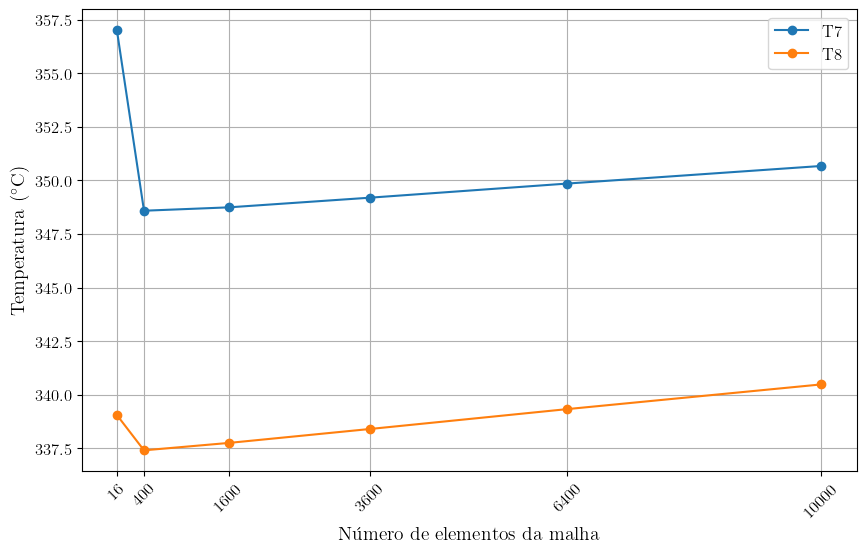
\includegraphics[width=0.8\textwidth]{Temps.png}
        \caption{Valores de temperatura obtidos com o refinamento da malha.}
        \label{fig:temp}
    \end{figure}
    \begin{figure}[p]
        \centering
        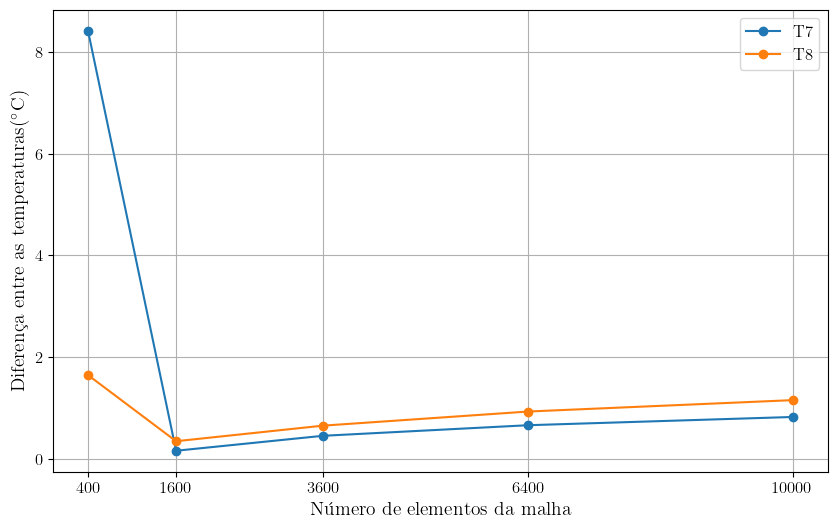
\includegraphics[width=0.8\textwidth]{Diff.png}
        \caption{Diferença entre temperaturas para número de elementos de malha distintos.}
        \label{fig:diff}
    \end{figure}
    \FloatBarrier
    \begin{figure}[htb]
        \centering
        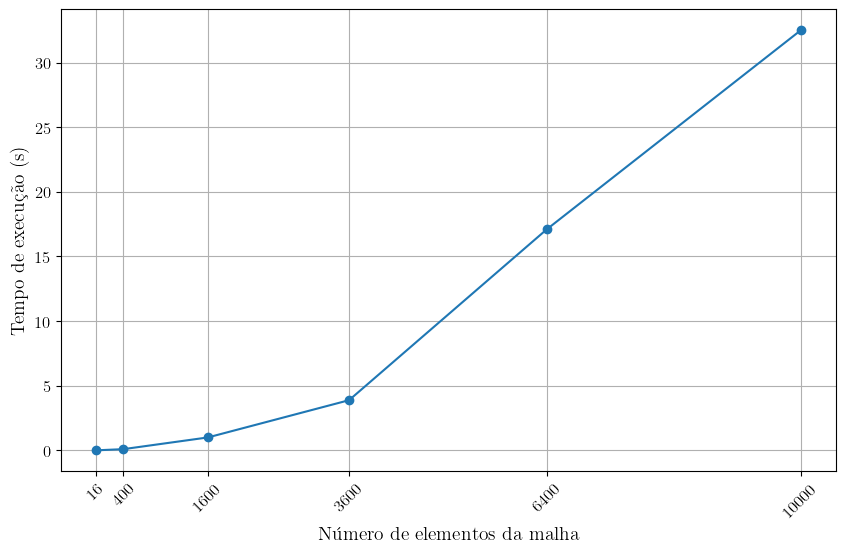
\includegraphics[width=0.8\textwidth]{Texec.png}
        \caption{Tempo de execução para diferentes números de elementos de malha.}
        \label{fig:texec}
    \end{figure}

    Portanto, o estudo de refino não nos permitiu selecionar uma configuração que caracterizasse a hipotese de independência de malha. Decidiu-se então, definir um critério de convergência consideravelmente restrito para as iterações que utilizam o método de Gauss-Seidel de forma a mimizar o erro de iterações e viabilizar a análise de refinamento de malha.

    A análise do critério de convergência $\varepsilon$ será feito no item \textbf{d)}

    \subsection*{Refino de malha com $\varepsilon = 10^{-8}\,^\circ\mathrm{C}$}
    Ao se realizar a nova análise, pôde-se notar que os valores de $\Delta T_7$ e $\Delta T_8$ se mostraram inferiores ao critério definido para independência de malha ($\Delta T \le 0,2\,^\circ\mathrm{C})$ já na segunda iteração ($n_{elementos} = 1600$ e $\Delta x = 0,025\,\mathrm{m}$.). Além disso, os resultados encontrados para as mesmas variáveis seguiram diminuindo à medida que $n_{elementos}$ crescia, o que demonstra uma tendência de convergência.
    Como o tempo de execução do método cresceu consideravelmente entre a terceira e a segunda iterações (um crescimento de aproximadamente 6 vezes), entende-se que a adoção da malha com 1600 pontos é a escolha que equilibra melhor a exatidão do resultado e o custo computacional.
    As temperaturas $T_7$ e $T_8$, calculadas para cada número de elementos de malha se encontram ilustradas na Figura ~\ref{fig:temp2}. Já os tempos computacionais, os números de malha adotados e as diferenças de temperatura $\Delta  T_7$ e $\Delta T_8$ se econtram na Tabela ~\ref{tab:tabe2} e nas Figuras ~\ref{fig:diff2} e ~\ref{fig:texec2}. A malha inicial ($n = 1$, $\Delta x = 0,25\,\mathrm{m}$, 16 elementos), correspondente à do Exemplo 4.3 do livro, serviu apenas como referência para o cálculo da primeira diferença de temperatura, não constando nas tabelas de $\Delta T$.

    \begin{table}[ht]
        \centering
        \caption{Diferenças de temperatura e tempos de execução para diversos números de elementos de malha.}
        \begin{tabular}{|c|c|c|c|}
        \hline
        n\degree\,elementos de malha & $\Delta T_7\,(^\circ\mathrm{C})$ & $\Delta T_8\,(^\circ\mathrm{C})$ & Tempo de execução (s) \\ \hline
        400   & 8,49   & 1,75   & 0,390  \\ \hline
        1600   & \textbf{0,11}   & \textbf{0,02}   & 6,181  \\ \hline
        3600   & 0,02   & 0,00   & 37,056  \\ \hline
        6400   & 0,01   & 0,00   & 106,981  \\ \hline
        10000   & 0,00   & 0,00   & 269,705  \\ \hline
        \end{tabular}
        \label{tab:tabe2}
    \end{table}
    \FloatBarrier
    
    \begin{figure}[p]
        \centering
        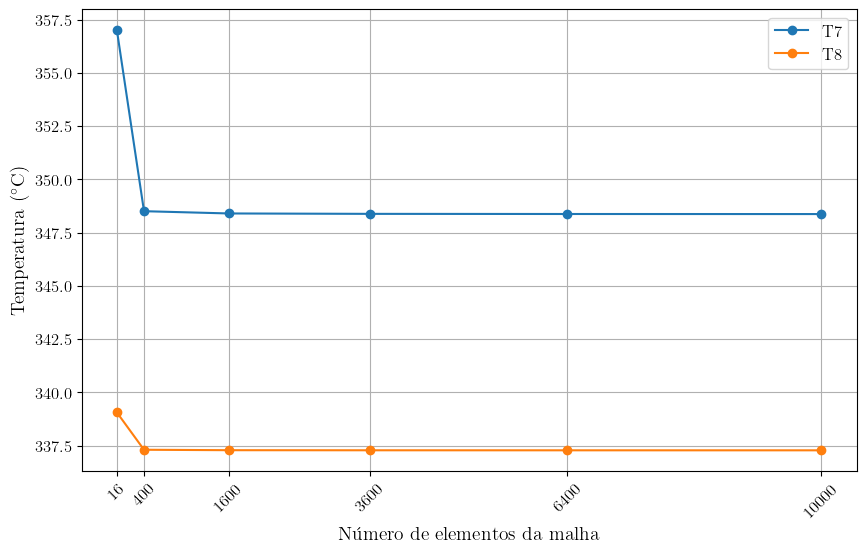
\includegraphics[width=0.8\textwidth]{Temps2.png}
        \caption{Valores de temperatura obtidos com o refinamento da malha.}
        \label{fig:temp2}
    \end{figure}
    \begin{figure}[p]
        \centering
        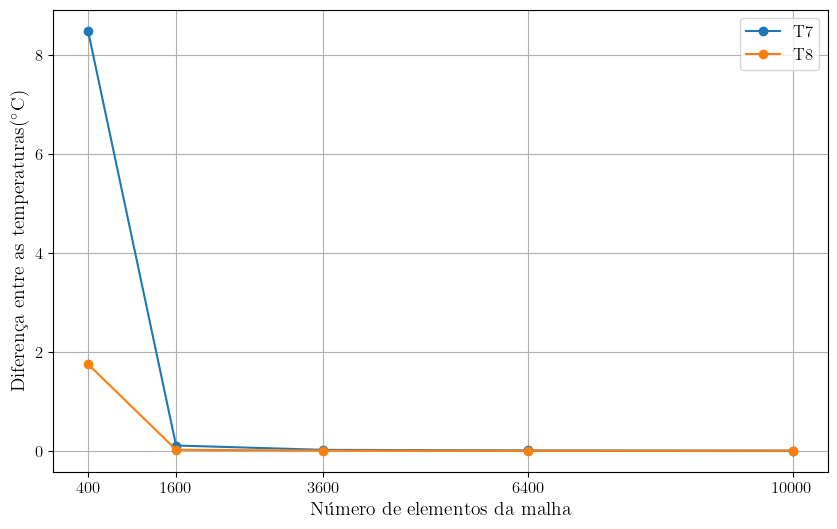
\includegraphics[width=0.8\textwidth]{Diff2.png}
        \caption{Diferença entre temperaturas para número de elementos de malha distintos.}
        \label{fig:diff2}
    \end{figure}
    \FloatBarrier
    \begin{figure}[htb]
        \centering
        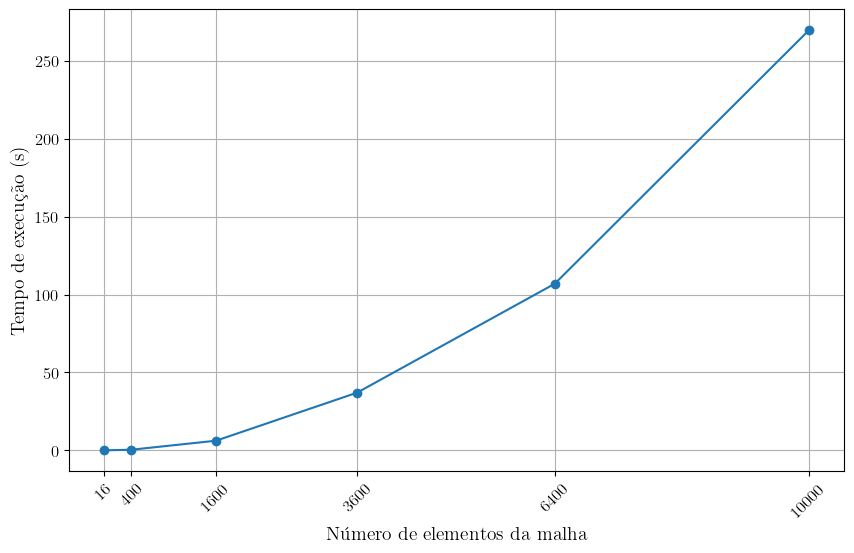
\includegraphics[width=0.8\textwidth]{Texec2.png}
        \caption{Tempo de execução para diferentes números de elementos de malha.}
        \label{fig:texec2}
    \end{figure}

    \item[d)]Após a seleção da malha, prosseguiu-se com a análise quanto ao critério de convergência ($\varepsilon$). Fixando-se a malha selecionada no item \textbf{c)} ($n_{elementos} = 1600$, $\Delta x = \Delta y = 0,025\,\mathrm{m}$), variou-se $\varepsilon$ utilizando a seguinte regra.
    
    \begin{center}
        $\varepsilon = 10^{-n}$ \quad $n = \{8, 7, \dots, 1\}$
    \end{center}

    Como o resultado obtido com $\varepsilon = 10^{-8}\,^\circ\mathrm{C}$ é, para efeitos práticos, a solução do sistema de equações algébricas associado a essa malha, adotou-se esse valor como referência e o erro de cada critério foi então definido como $|T_i(\varepsilon) - T_i(10^{-8})|$, o que permite quantificar diretamente a perda de exatidão decorrente da adoção de critérios menos restritivos. O ponto de referência não consta do gráfico de erros, uma vez que seu desvio em relação a si mesmo é nulo por
    definição.

    A Figura~\ref{fig:temps3} apresenta os valores de $T_7$ e $T_8$ obtidos para cada critério. Ambas as temperaturas permaneceram praticamente constantes para $\varepsilon \le 10^{-3}\,^\circ\mathrm{C}$, afastando-se de forma perceptível apenas nos dois critérios mais frouxos.

    \begin{figure}[htb]
        \centering
        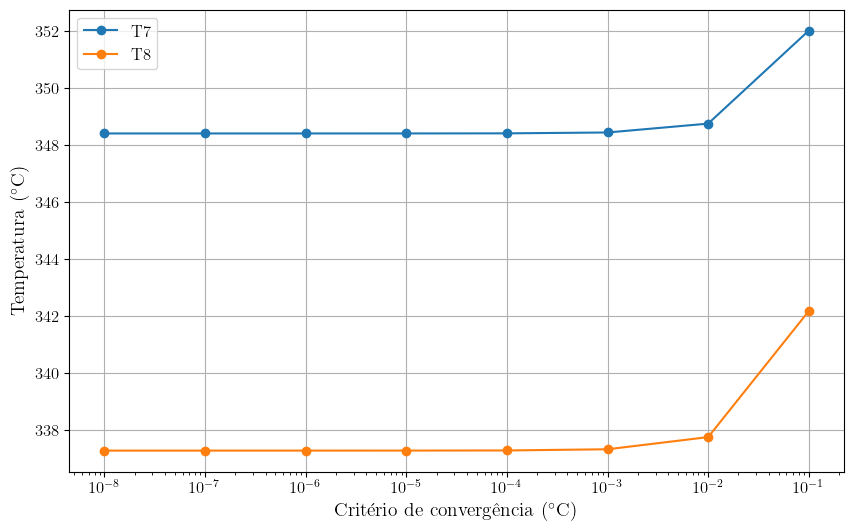
\includegraphics[width=0.8\textwidth]{Temps3.png}
        \caption{Valores de temperatura obtidos para critérios de convergência distintos.}
        \label{fig:temps3}
    \end{figure}
    \FloatBarrier

    A Figura~\ref{fig:diff3} apresenta o erro em relação à referência em escala logarítmica em ambos os eixos. A adoção dessa escala se justifica pela amplitude dos valores de erro obtidos (de $3,03\times10^{-6}$ a $3,60\,^\circ\mathrm{C}$).

    A partir da análise da Tabela~\ref{tab:tabe3} e da Figura~\ref{fig:diff3}, cabe-se notar que o critério de convergência $\varepsilon = 10^{-3}\,^\circ\mathrm{C}$ atende o limite previamente adotado para a hipótese de independência de malha $\Delta T \le 0,2\;^\circ\mathrm{C}$ 


    \begin{table}[ht]
        \centering
        \caption{Diferenças de temperatura e tempos de execução para diferentes critérios de convergência}
        \begin{tabular}{|c|c|c|c|}
        \hline
        $\varepsilon\,(^\circ\mathrm{C})$ & $|T_7(\varepsilon) - T_7(10^{-8})|$ & $|T_8(\varepsilon) - T_8(10^{-8})|$ & Tempo de execução (s) \\ \hline
        $10^{-7}$   & $3,03\times10^{-6}$  & $4,16\times10^{-6}$   & 5,588  \\ \hline
        $10^{-6}$   & $3,31\times10^{-5}$    & $4,56\times10^{-5}$   & 4,870  \\ \hline
        $10^{-5}$   & $3,35\times10^{-4}$   & $4,61\times10^{-4}$    & 3,992  \\ \hline
        $10^{-4}$   & $3,34\times10^{-3}$   & $4,60\times10^{-3}$    & 2,376  \\ \hline
        $10^{-3}$   & $0,03$   & $0,05$   & 1,780  \\ \hline
        $10^{-2}$   & $0,33$   & $0,47$   & 0,974  \\ \hline
        $10^{-1}$   & $3,60$   & $4,89$   & 0,303  \\ \hline
        \end{tabular}
        \label{tab:tabe3}
    \end{table}
    \FloatBarrier

    \begin{figure}[htb]
        \centering
        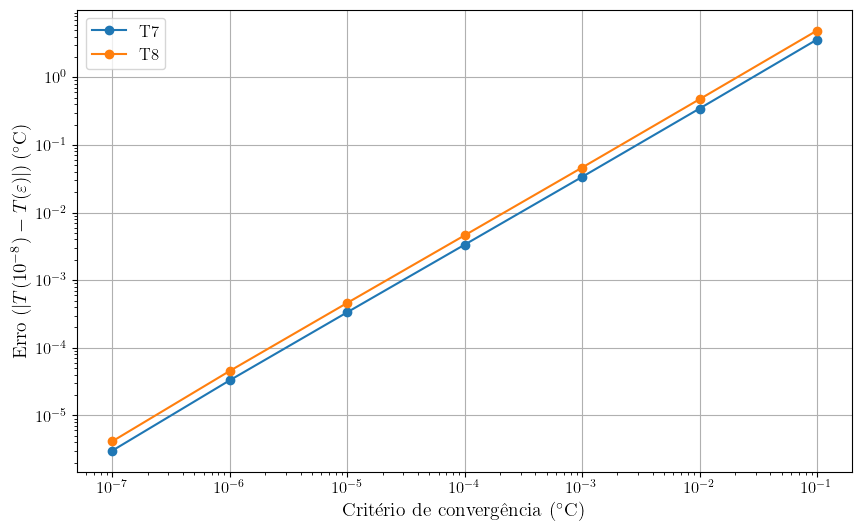
\includegraphics[width=0.8\textwidth]{Diff3.png}
        \caption{Diferença entre temperaturas para critérios de convergência distintos.}
        \label{fig:diff3}
    \end{figure}
    \FloatBarrier

    Além disso, ao avaliar os tempos de execução do método, nota-se que, para $\varepsilon = 10^{-3}\,^\circ\mathrm{C}$, o tempo de execução não se mostra excessivamente custoso (aproximadamente 32\% daquele obtido quando se utilizado $\varepsilon = 10^{-8}\,^\circ\mathrm{C}$). Conforme observado na Tabela~\ref{tab:tabe3} e na Figura~\ref{fig:texec3}.

    \begin{figure}[htb]
        \centering
        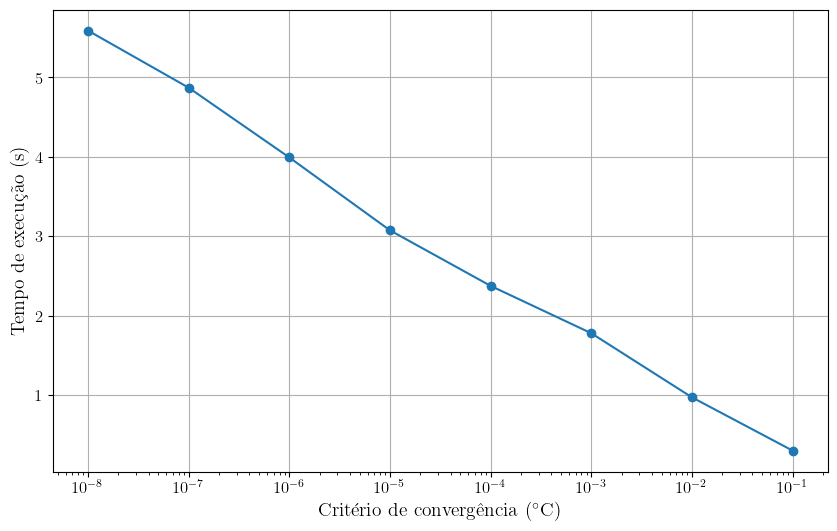
\includegraphics[width=0.8\textwidth]{Texec3.png}
        \caption{Tempos de execução para critérios de convergência distintos}
        \label{fig:texec3}
    \end{figure}
    \FloatBarrier

    \item[e) ] A Figura~\ref{fig:temp3d} mostra o gráfico 3D da distribuição de temperaturas obtidas no problema a partir da escolha da malha com $n_{elementos} = 1600$ e com o critério de convergência $\varepsilon = 10^{-3}$
    
    \begin{figure}[htb]
        \centering
        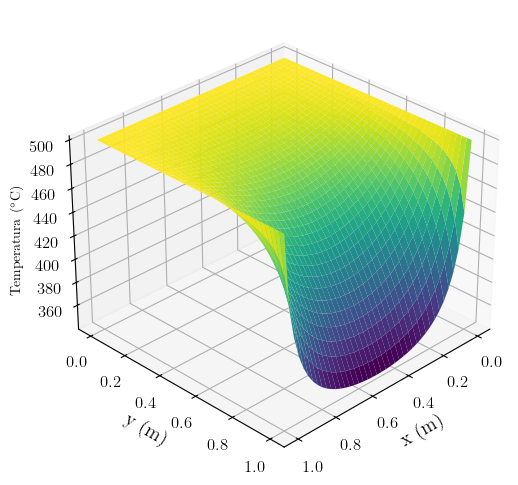
\includegraphics[width=0.8\textwidth]{3Dtemp.png}
        \caption{Campo de temperaturas}
        \label{fig:temp3d}
    \end{figure}
    \FloatBarrier

    \item[f) ]A Figura~\ref{fig:3dflux} mostra o gráfico de vetores do fluxo de calor a partir da distribuição de temperaturas obtidas no problema a partir da escolha da malha com $n_{elementos} = 1600$ e com o critério de convergência $\varepsilon = 10^{-3}$
    
    \begin{figure}[t]
        \centering
        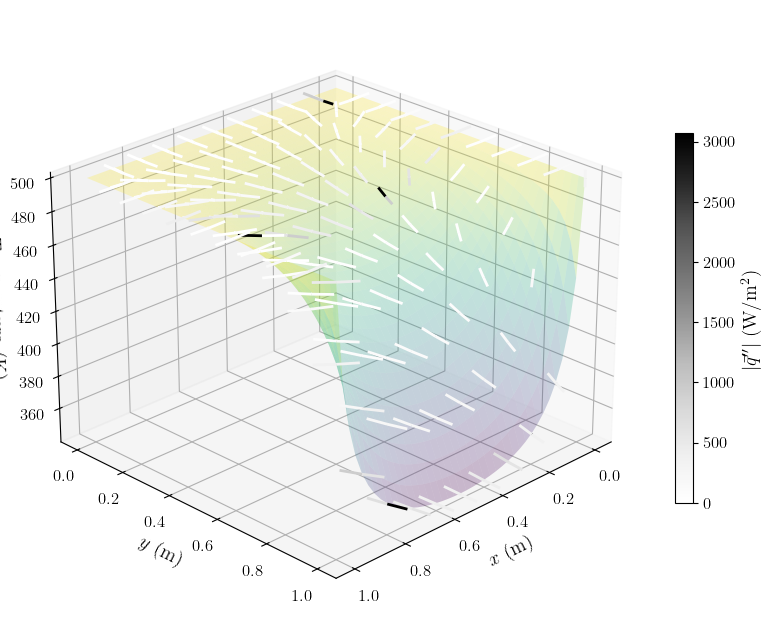
\includegraphics[width=0.8\textwidth]{3dFlux.png}
        \caption{Campo de temperaturas}
        \label{fig:3dflux}
    \end{figure}
    \FloatBarrier

\end{itemize}